\documentclass[12pt]{article}

\usepackage{amsmath}
\usepackage{amssymb}
\usepackage{amsthm}
\usepackage{fullpage}
\usepackage{makecell}
\usepackage{tabularx}

\usepackage[dvipsnames]{xcolor}
\usepackage{tikz,tkz-euclide}
\usetikzlibrary{decorations.pathreplacing}
\usetikzlibrary{quotes,angles,calc,intersections}

\usepackage{titling}
\usepackage{pdfpages}
\usepackage{color}
\usepackage{hyperref}

\usepackage{common}
\usepackage{linear}

\begin{document}

\title{Vector Calculus Notes}
\author{Brendan Burkhart}
\maketitle

\tableofcontents
\newpage

\section{Orthogonal Projection}

\begin{figure}[ht!]
    \centering
    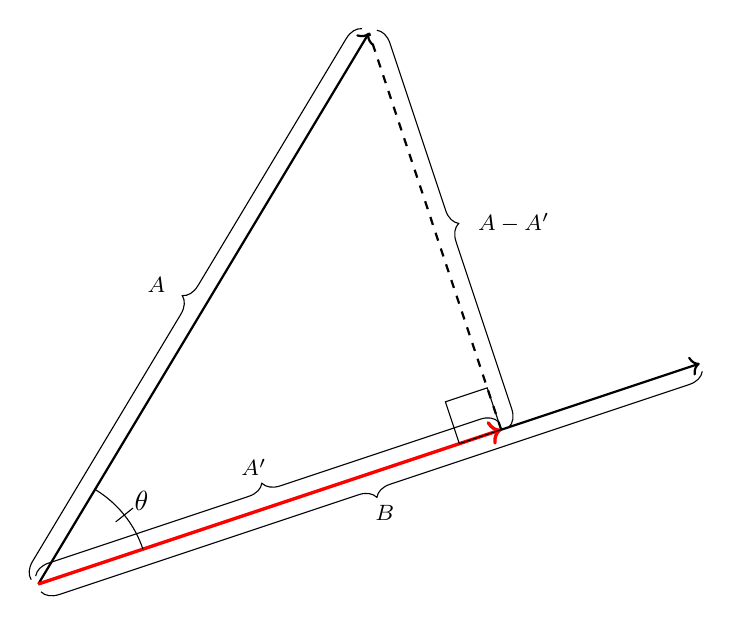
\begin{tikzpicture}[scale=1.4]
        \coordinate (O) at (0, 0);
        \coordinate (A) at (3, 5);
        \coordinate (B) at (6, 2);
        \coordinate (A') at ($(O)!(A)!(B)$);

        \draw [thick, ->] (O) -- (A);
        \draw [thick, ->] (O) -- (B);
        \draw [thick, dashed] (A') -- (A);
        \draw [very thick, red, ->] (O) -- (A');

        \draw [decorate,decoration={brace,amplitude=6pt,raise=3pt]}]
            (O) -- (A) node [black,midway,xshift=-0.6cm,yshift=0.3cm]
            {\footnotesize $A$};

        \draw [decorate,decoration={brace,amplitude=6pt,raise=3pt]}]
            (B) -- (O) node [black,midway,xshift=0.2cm,yshift=-0.5cm]
            {\footnotesize $B$};

        \draw [decorate,decoration={brace,amplitude=6pt,raise=3pt]}]
            (A) -- (A') node [black,midway,xshift=1.0cm, yshift=0.1cm]
            {\footnotesize $A - A'$};

        \draw [decorate,decoration={brace,amplitude=6pt,raise=3pt]}]
            (O) -- (A') node [black,midway,xshift=-0.2cm, yshift=0.5cm]
            {\footnotesize $A'$};

        \tkzMarkAngle[size=1cm,mark=|](B,O,A)
        \tkzLabelAngle[pos=1.2](B,O,A) {$\theta$}

        \tkzMarkRightAngle[size=0.4](A,A',O)
    \end{tikzpicture}
\caption{Orthogonal projection of $\vec{A}$ onto $\vec{B}$}
\label{fig:orthogonal-projection}
\end{figure}

Figure \ref{fig:orthogonal-projection} shows $A'$, the orthogonal projection of vector $A$ onto $B$. $\norm{A'}$ is the shortest distance between the head of $A$ and $B$.

\begin{thm}
    Let $\theta$ be the angle between non-zero vectors $A$ and $B$. Then $\cos\theta = \frac{A \cdot B}{\norm{A}\norm{B}}$.
\end{thm}

\begin{proof}\label{vector-angle}
    Let $C = A - B$. Then $C \cdot C = (A - B) \cdot (A - B)$, which can we expand to get $A \cdot (A - B) - B \cdot (A - B) = A \cdot A + B \cdot B - 2(A \cdot B)$. Therefore, $\norm{C}^2 = \norm{A}^2 + \norm{B}^2 - 2(A \cdot B)$. By the Law of Cosines, $A \cdot B = \norm{A}\norm{B}\cos\theta$, so $\cos\theta = \frac{A \cdot B}{\norm{A}\norm{B}}$.
\end{proof}

\begin{exmp}
    Let $A = \left(0, 1\right)$, and $B = \left(2, 2\right)$. Then $\cos\theta = \frac{A \cdot B}{\norm{A}\norm{B}}$. Since $A \cdot B = 0 \cdot 2 + 1 \cdot 2 = 2$, $\norm{A} = \sqrt{0^2 + 1^2} = 1$, and $\norm{B} = \sqrt{2^2 + 2^2} = \sqrt{8} = 2\sqrt{2}$, we have $\cos\theta = \frac{2}{1 \cdot 2\sqrt{2}}$. This is equal to $\frac{\sqrt{2}}{2}$, so $\theta = \frac{\pi}{4}$.
\end{exmp}

\begin{exmp}
    Let $A = {1, 1}$ and $B = {1, -1}$. Then since $A \cdot B = 1 - 1 = 0$, we know $\cos\theta = 0$, which implies that $\theta = \frac{\pi}{2}$.
\end{exmp}

\begin{cor}\label{perpendicular-vectors}
    In general, non-zero $A$ and $B$ are perpendicular if and only if $A \cdot B = 0$.
\end{cor}

\begin{proof}
    Let $A$ and $B$ be non-zero perpendicular vectors. Then the angle ($\theta$) between $A$ and $B$ must be $\frac{\pi}{2}$ since they are perpendicular. By Theorem \ref{vector-angle}, $\cos\theta = \frac{A \cdot B}{\norm{A}\norm{B}}$. Since $A$ and $B$ are non-zero, $\norm{A}\norm{B}$ is non-zero, and since $\theta = \frac{\pi}{2}$, we know $\cos\theta = 0$. Therefore, $A \cdot B$ must equal zero.
\end{proof}

\begin{thm}\label{vector-projection}
    Let $A$ and $B$ be vectors, and $A'$ be the orthogonal projection of $A$ onto $B$. Then $A' = \frac{A \cdot B}{B \cdot B}B$.
\end{thm}

\begin{proof}
    Let $d \in \R$ such that $C = dB$. Then since $(A - dB) \cdot B = 0$, we know $A \cdot B - dB \cdot B = 0$, so $A \cdot B = d(B \cdot B)$. This implies that $d = \frac{A \cdot B}{B \cdot B}$. Since $C = dB$, we then have $C = \frac{A \cdot B}{B \cdot B}B$.
\end{proof}

\begin{exmp}
   Let $A = \left(2, 2\right)$, and $B = \left(1, 0\right)$. Then since $A \cdot B = 2$, and $B \cdot B = 1$, we know $A' = \frac{2}{1}B = \left(2, 0\right)$.
\end{exmp}

\section{Cross Product}

\begin{defn}
    The \emph{cross product} or \emph{vector product} of three-dimensional vectors $A = a_1i + a_2j + a_3k$ and $B = b_1i + b_2j + b_3k$ is written $A \times B$. \[A \times B = \begin{vmatrix}
        i & j & k \\ a_1 & a_2 & a_3 \\ b_1 & b_2 & b_3
    \end{vmatrix}\] The value of this determinant can be found via the Laplace formula (also called cofactor expansion) along any column or row. Expansion along the first row gives: \[A \times B =
    \begin{vmatrix}
        i & j & k \\ a_1 & a_2 & a_3 \\ b_1 & b_2 & b_3
    \end{vmatrix} =
    \begin{vmatrix}
        a_2 & a_3 \\ b_2 & b_3
    \end{vmatrix}i -
    \begin{vmatrix}
        a_1 & a_3 \\ b_1 & b_3
    \end{vmatrix}j +
    \begin{vmatrix}
        a_1 & a_2 \\ b_1 & b_2
    \end{vmatrix}k\] \[= (a_2b_3 - b_2a_3)i - (a_1b_3 - b_1a_3)j + (a_1b_2 - b_1a_2)k.\]
\end{defn}

\begin{rmk}
    The cross product is a non-commutative binary operation.
\end{rmk}

\begin{exmp}
    Let $A = 3i + j - k$, and $B = -6i - 2j - 2k$. Then \[A \times B =
    \begin{vmatrix}
        i & j & k \\ 3 & 1 & -1 \\ -6 & -2 & -2
    \end{vmatrix} = (-2 - 2)i - (-6 - 6)j + (-6 + 6)k = -4i + 12j + 0k.\]
\end{exmp}

\begin{thm}
    Let $A = a_1i + a_2j + a_3k$ and $B = b_1i + b_2j + b_3k$ be vectors. Then $A \times B$ is perpendicular to both $A$ and $B$.
\end{thm}

\begin{proof}
    Since $A \times B = (a_2b_3 - b_2a_3)i - (a_1b_3 - b_1a_3)j + (a_1b_2 - b_1a_2)k$, we know that $A \cdot (A \times B) = (a_1a_2b_3 - a_1b_2a_3) - (a_1a_2b_3 - b_1a_2a_3) + (a_1b_2a_3 - b_1a_2a_3)$. This is equal to $(a_1a_2b_3 - a_1a_2b_3) - (b_1a_2a_3 - b_1a_2a_3) + (a_1b_2a_3 - a_1b_2a_3)$, which is equal to $0$, so by Corollary \ref{perpendicular-vectors} we know $A$ is perpendicular to $A \times B$. Similarly, $B$ is perpendicular to $A \times B$.
\end{proof}

\begin{thm}
    Let $A$, $B$, and $C$ be vectors, and $x$ a real number. Then:
    \begin{itemize}
        \item $A \times B = 0$ if and only if $A = \vec{0}$ or $B = \vec{0})$, or $A$ is parallel to $B$.
        \item $A \times B = -(B \times A)$.
        \item $A \times (B + C) = (A \times B) + (A \times C)$.
        \item $(A + B) \times C = (A \times C) + (B \times C)$.
        \item $(\alpha A) \times B = A \times (\alpha B) = \alpha(A \times B)$.
    \end{itemize}
\end{thm}

\begin{proof}
    
\end{proof}

\begin{rmk}
    In a \emph{right-handed} coordinate system, the cross product will follow the \emph{right-hand rule}: on the right hand, index finger represents $A$, middle finger represents $B$, and then thumb represents $A \times B$. However, in a \emph{left-handed} coordinate system, the cross product will instead follow the similar \emph{left-hand rule}. The chirality of the cross product follows the chirality of the chosen basis, and is not inherently due to the definition of the cross product.
\end{rmk}

\begin{thm}
    Let $A$ and $B$ be two vectors, and $\theta$ be the angle between them. Then $\norm{A \times B} = \norm{A}\norm{B}\sin\theta$, which is the area of a parallelogram with side lengths $\norm{A}$ and $\norm{B}$ and angle $\theta$.
\end{thm}

\begin{thm}
    Let $(x_1, y_1, z_1)$ be a point, and $Ax + By + Cz + D = 0$ be a plane. Then the distance from the point to the plane is: \[\frac{\abs{Ax_1 + By_1 + Cz_1 + D}}{\sqrt{A^2 + B^2 + C^2}}.\]
\end{thm}

\begin{proof}
    The line with direction $(A, B, C)$ that passes through the point is normal to the plane and thus contains the shortest path from the point to the plane. Therefore, $A(x_1 + At) + B(y_1 + Bt) + C(z_1 + Ct) + D = 0$ gives the closest point on the plane to the point. $Ax_1 + By_1 + Cz_1 + D = -t(A^2 + B^2 + C^2)$. The shortest distance is thus \[\abs{\frac{t}{\norm{(A, B, C)}}} = \frac{\abs{Ax_1 + By_1 + Cz_1 + D}}{\sqrt{A^2 + B^2 + C^2}}.\]
\end{proof}

\end{document}
